\documentclass[tikz]{standalone}
\usepackage{pgfplots}
\pgfplotsset{compat=1.15}
\usepackage{mathrsfs}
\usetikzlibrary{arrows,calc}
\usepackage{tkz-euclide}
\pagestyle{empty}

\definecolor{AngleClr}{rgb}{0,0.39215686274509803,0}
\definecolor{ShapeClr}{rgb}{0.6,0.2,0}

\begin{document}

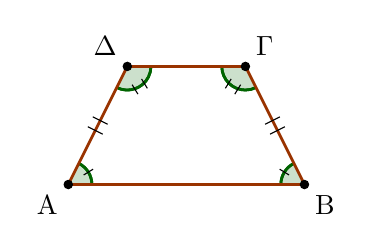
\begin{tikzpicture}[scale=.75]
\tkzSetUpLine[line width=1pt,color=black]
\tkzSetUpPoint[fill=black]

\tkzDefPoints{0/0/A,4/0/B,1/2/D,3/2/C}

\tkzFillPolygon[fill=white](A,B,C,D)

\tkzFillAngles[fill=AngleClr,size=.4,fill opacity=0.2](A,D,C D,C,B B,A,D C,B,A)
\tkzMarkAngles[line width=1pt,color=AngleClr,size=.4](A,D,C D,C,B B,A,D C,B,A)
\tkzMarkAngles[mark=||,mksize=2,line width=1pt,size=.4,color=AngleClr](A,D,C D,C,B)
\tkzMarkAngles[mark=|,mksize=2,line width=1pt,size=.4,color=AngleClr](B,A,D C,B,A)

\tkzDrawPolygon[color=ShapeClr](A,B,C,D)
\tkzDrawPoints[size=3](A,B,C,D)
\tkzLabelPoint[below left](A){$\rm A$}
\tkzLabelPoint[below right](B){$\rm B$}
\tkzLabelPoint[above right](C){$\rm \Gamma$}
\tkzLabelPoint[above left](D){$\rm \Delta$}

\tkzMarkSegments[mark=||,size=3](A,D B,C)

\end{tikzpicture}
\end{document}
